\chapter{Chrome擴充套件設計與實作}
\indent

在一個已經寫好自動化腳本的網頁下,
若更改了HTML中裡面的元件結構變化,
舊有的XPath有可能會無法定位元件從而導致腳本錯誤。
為了提高XPath的穩定性,路徑表達式在設計時通常會盡量不強制指定節點階層且使用更改頻率較低的元件屬性來當作路徑條件,
藉此來避免調整HTML架構後無法抓取網頁中的元件。

本論文以呂昭陞``提出提升穩定性的XPath撰寫樣式''論文\cite{LIU-Thesis}中的觀念為基礎,尋找符合的路徑條件並撰寫出穩定性高的網頁測試腳本,
但在設計XPath中,找出好的路徑條件,對測試人員來說是需要對該網頁有一定的認識且有相關經驗才比較容易做到的。
因此本論文提出在測試人員需要找尋適合的條件的時候,
可以透過Chrome擴充套件增加比較HTML文檔和過濾自訂屬性等等額外功能的設計,
讓測試人員即使在大型的HTML架構中也可以篩選掉大部分的元件,
從中選出適合的元件屬性來作為路徑條件,撰寫能準確定位該元件且穩定性高的XPath表達式。

% =========================================================================================
% =========================================================================================
\section{擴充元件之使用情境}\label{s3.1}
\subsection{設計互動元件XPath路徑條件}\label{s3.1.1}
在章節\ref{s2.4}有提到XPath的組成方式,分別是Axis、Node test和零個或多個Predicate。
為了確保表達式中的穩定性,通常在設計時,會同時使用這三種元件來組成一個路徑表達式。

在撰寫測試腳本時,每做完一個元件互動後,
通常都需要驗證有相互關係的元件有出現或消失以確保該元件的互動行為有確實被執行,
這時可以利用元件屬性的變化或元件的增減當成XPath的限制條件,
若畫面沒有執行元件互動後的互動形為,代表XPath中設定的條件無法達成,從而導致元件無法成功定位。
換句話說,若使用者要用XPath表達式來判斷是否互動成功,可以找出變化並將變化加入XPath的路徑條件中。

以圖\ref{f3.1}舉例,
點擊了按鈕後,
HTML中會發現div元件中的class會從``status-one''變成``status-two'',
若要用XPath表達式來確保成功點擊按鈕,
可以撰寫成\colorbox{lightgray}{//div[@class=``status-two'']//p[text()=``Status msg'']},
如果網頁有問題,互動後元件中的class屬性沒有改變的話,
上述XPath中\colorbox{lightgray}{@class=``status-two''}的條件會無法符合,
即無法定位到該元件位置,導致測試腳本執行失敗。

\begin{figure}[H]
    \centering
    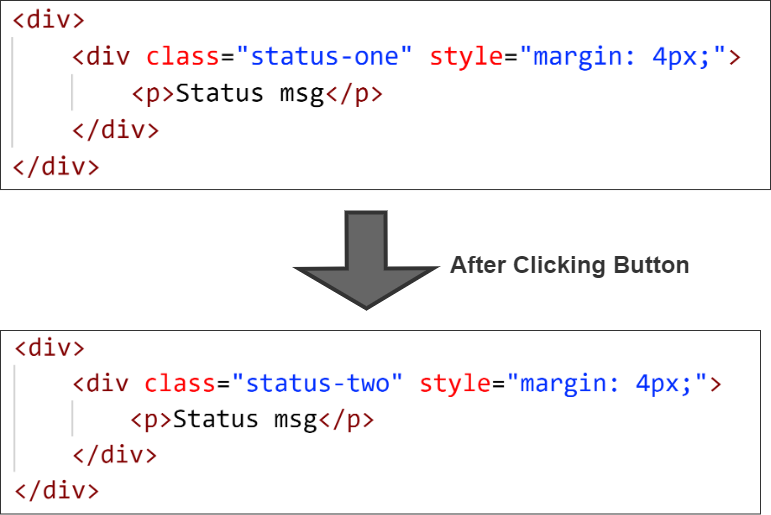
\includegraphics[width=0.6\textwidth]{picture/ch3-html-after-change.png}
    \caption{互動後HTML改變之範例圖}
    \label{f3.1}
\end{figure}

由上述例子可知,HTML變化後的元件或元件屬性很適合在測試腳本中當作判斷互動是否成功的依據。
一般使用者若需要查看當下網頁中的HTML,會打開瀏覽器中的Developer Tools,
藉由Developer Tools中``Inspect Element''功能,直接跳轉到使用者點選物件的HTML位置來查看元件的變化。
使用者在尋找元件變化的時候,常常會遇到元件互動時HTML快速變化和HTML多層元件未展開無變化提示兩種情形。

\subsection{元件互動時HTML快速變化}\label{s3.1.2}

使用者在網頁中元件有互動行為時,
可以在Developer Tools中發現部分元件的內容或屬性會因為互動而產生快速的變化。
如圖\ref{f3.2}所示,變化的元件會有紫色的漸淡背景框來提醒使用者。
通常在元件屬性比較冗長複雜的情況下,
元件的快速變化會造成使用者無法立即觀察出變化,
需要花較長的時間重複元件互動行為來判斷其中的差異。

\begin{figure}[H]
    \centering
    \includegraphics[width=1.0\textwidth]{picture/ch3-element-change-fast.png}
    \caption{HTML互動後元件變化之顯示}
    \label{f3.2}
\end{figure}

\subsection{HTML多層元件未展開無變化提示}\label{s3.1.3}

通常使用者會利用Developer Tools中``Inspect Element''功能來找出元件在HTML中的位置,
在使用這個功能時,會自動展開該元件上層的所有直屬元件,
因為它只會展開直屬元件,
若未展開的元件或在Developer Tools中Element頁面需要滾動才看的元件有變化的話,
容易會被使用者忽略,
以圖\ref{f3.3}為例,
左半部的圖是未展開的狀態,在未展開時,紅色框內的元件並沒有紫色的漸淡背景框,
但和右半部的圖一樣把元件展開後,會發現裡面確實有元件在變化並且有紫色的漸淡背景框來提示使用者。

\begin{figure}[H]
    \centering
    \includegraphics[width=1.0\textwidth]{picture/ch3-element-change-nghide.png}
    \caption{HTML未展開導致不會顯示變化提示}
    \label{f3.3}
\end{figure}

\subsection{使用擴充工具之原因}\label{s3.1.4}
因為章節\ref{s3.1.3}和章節\ref{s3.1.4}敘述的兩種情況,
導致僅靠Developer Tools找出變化會花較長時間,
在此情況下可以使用此工具利用HTML比較的方式把HTML中相異的地方列出,
讓測試人員藉由工具所列出的差異來設計XPath,從而減少挑選路徑條件的時間。

% =========================================================================================
% =========================================================================================
\section{系統架構}\label{s3.2}
圖\ref{f3.4}為Chrome擴充套件實作的系統架構圖,下列為各元件之介紹:

\begin{itemize}
\item\textbf{Chrome:}
以市占率第一的Chrome瀏覽器為背景下,對瀏覽器擴充元件進行實作

\item\textbf{Chrome Extension: }
以Chrome瀏覽器的情形下,基於原始的瀏覽器功能下,增加自定義功能到瀏覽器之瀏覽器擴充程式

\item\textbf{Background Script For Extension: }
擴充程式腳本之一, 屬於擴充元件的背景程序,通常會將擴充程式的主要邏輯放在此腳本中

\item\textbf{SidePanel Script For Extension: }
擴充程式腳本之一, 在擴充元件Element頁面下的子頁面

\item\textbf{HTML Compare Function: }
比對兩個HTML差異之程式模組

\item\textbf{UI Interface: }
擴充元件在SidePanel裡面的使用者介面設計

\item\textbf{Test Script: }
針對Compare Function的單位測試腳本

\end{itemize}

\begin{figure}[H]
    \centering
    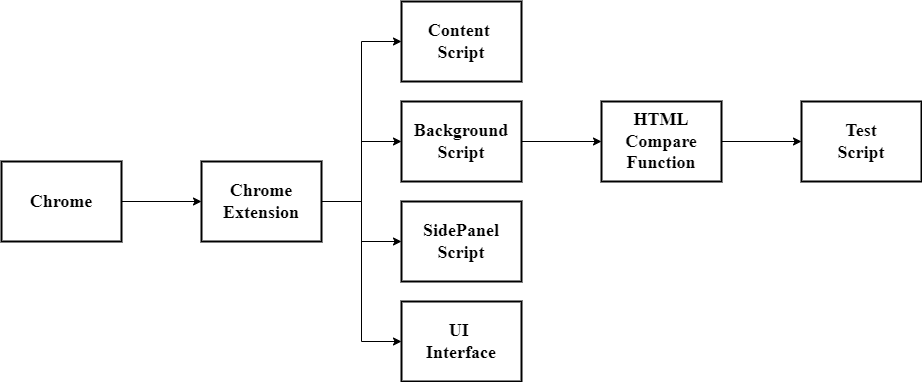
\includegraphics[width=0.9\textwidth]{picture/ch3-systemStucture.png}
    \caption{擴充元件實作之架構圖}
    \label{f3.4}
\end{figure}

此設計架構主要是以HTML比對函數為主,
利用多個Chrome Extension的專用腳本,
讀出網頁的HTML並丟入比對函數中,最後利用UI介面把結果顯示在畫面上。

% =========================================================================================
% =========================================================================================
\section{HTML比對之實作}\label{s3.3}
此工具所採用的方法為對整個網頁來進行比對,並標示出相異的結果,
若僅僅只有觀察特定物件的變化,可能會忽略HTML中上方或下方其他更適合當條件的元件,以至於較難設計XPath表達式。
如果需要查看特定物件的變化,可以使用章節\ref{s3.5.3}中提到的``Only display change of current selecting elemnt''功能。

一般在做比對時,會使用基本的Diff文本比對演算法來顯示差異的結果,
但對於HTML來說,藉由XML中的結構特性,
可以解析每個節點的屬性和特徵,
讓結果可以調整成更趨近使用者期望的狀況,
可以使比對產生的誤報較少,未來若需要額外添加比對限制也較為容易,
因此採用專門針對HTML設計的比對演算法。
在進行HTML比對之前,需要先取出網頁互動前後的兩個HTML,然後再開始執行HTML比對\cite{HTML-Comparison-Algorithm}。
此比對實作使用了開源程式Hiff\cite{Hiff}的架構,經過權重部分修改、輸出元件的調整以及增加相關功能的單元測試,
調整成適合擴充程式的內部核心程式,並將此實作放入擴充程式的Background Script中。圖\ref{f3.5}為HTML比對之活動圖。

\begin{figure}[H]
    \centering
    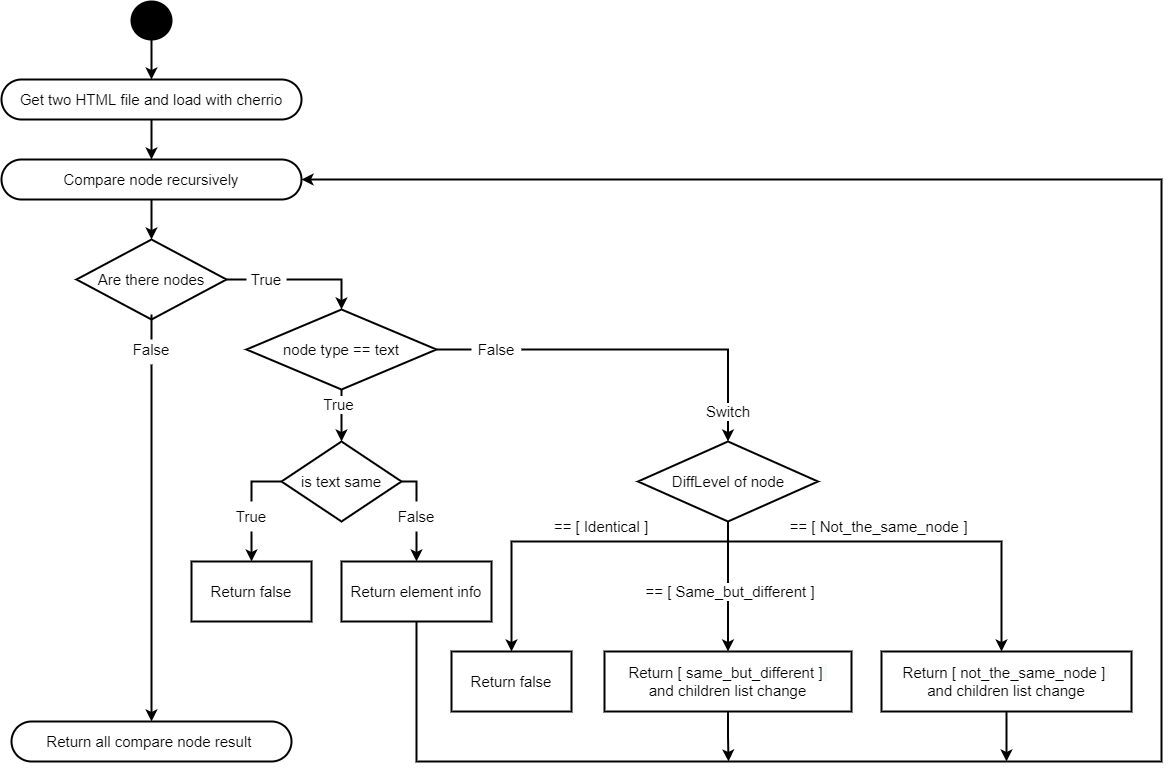
\includegraphics[width=1.0\textwidth]{picture/ch3-activity diagram.png}
    \caption{HTML比對之活動圖}
    \label{f3.5}
\end{figure}

\subsection{判斷節點相異程度}\label{s3.3.1}
在兩個HTML節點的相互比對中,需先判斷它們的相異程度,才能進一步的知道元件變化的類型,
可以將相異程度分成三個等級:Identical、Same but different和Not the same node。
圖\ref{f3.6}為本程式的實作流程,
會先做各屬性的比對,然後根據當前狀況選擇要該屬性自定義的權重,
最後將所有權重相加來判斷節點相異等級。

\begin{figure}[H]
    \centering
    \includegraphics[width=1.0\textwidth]{picture/ch3-HEURISTIC-comapre.png}
    \caption{節點相異程度之活動圖}
    \label{f3.6}
\end{figure}

\subsection{比對輸出結果}\label{s3.3.2}
在比對中可以將相異的元件分成三種類型:Changed、Added和Removed,
三種類型皆需要回傳相對應的資訊。
舊有的開源程式碼僅只有對該變更資訊用字串加上顏色標記來告訴使用者變更結果,
經過修改後,額外在回傳的物件中添加了變更節點的解析資訊以及詳細屬性變化資訊,
在SidePanel Script中可以將比對函式回傳的結果直接取用,避免其他的腳本對回傳結果做額外處理。

程式碼\ref{l3.1}為changed類型的輸出結果,
其中除了回傳解析後的節點資訊,
裡面``info-compare''的值為比對該變化元件的所有類別結果,包括比對前、比對後和差異結果。

\begin{lstlisting}[caption=比對輸出結果(changed類型), label={l3.1}]
    1   function changed($nodeBefore, $nodeAfter) 
    2   {
    3    var before = grabParentAndIndex($nodeBefore),
    4    after = grabParentAndIndex($nodeAfter);
    5
    6    return {
    7    type: "changed",
    8    before:locationInfo(before.$parent, $nodeBefore, before.index),
    9    after: locationInfo(after.$parent, $nodeAfter, after.index),
    10   selectingNode: $nodeAfter,
    11   nodeINFO: $nodeBefore,
    12   info-compare: info_compare ($nodeBefore, $nodeAfter)
    13   };
    14  }
\end{lstlisting}

程式碼\ref{l3.2}和程式碼\ref{l3.3}為added和changed類型的輸出結果,
其中除了回傳解析後的相關節點資訊,
裡面``contentHTML''的值為added或removed元件的內部HTML資訊,會在UI介面中將整個變更的區塊告訴使用者。

\begin{lstlisting}[caption=比對輸出結果(added類型), label={l3.2}]
    1   function added($addedNode, $parentBefore, indexBefore, 
    2       $parentAfter, indexAfter) 
    3   {
    4     return {
    5     type: "added",
    6     before: locationInfo($parentBefore, undefined, indexBefore),
    7     after:  locationInfo($parentAfter, $addedNode, indexAfter),
    8     selectingNode: $parentAfter,
    9     nodeINFO: $addedNode,
    10    contentHTML: stringify($addedNode, false),
    11    };
    12  }
\end{lstlisting}

\begin{lstlisting}[caption=比對輸出結果(removed類型), label={l3.3}]
    1   function removed($removedNode, $parentBefore, indexBefore, 
    2       $parentAfter, indexAfter) 
    3   {
    4    return {
    5    type: "removed",
    6    before: locationInfo($parentBefore, $removedNode, indexBefore),
    7    after:  locationInfo($parentAfter, undefined, indexAfter),
    8    selectingNode: $parentAfter,
    9    nodeINFO: $removedNode,
    10   contentHTML: stringify($removedNode, false),
    11   };
    12  }
\end{lstlisting}


% =========================================================================================
% =========================================================================================
\section{擴充元件腳本設計之實作}\label{s3.4}
\indent
在章節\ref{s2.6.3}中已對不同類型的腳本做基本介紹,針對各腳本獨特的特性分配它需要執行的功能。
圖\ref{f3.7}中表示執行功能後的執行順序及流程,從按下比對按鈕到比對結束的內部腳本溝通流程圖。

\indent

\begin{figure}[H]
    \centering
    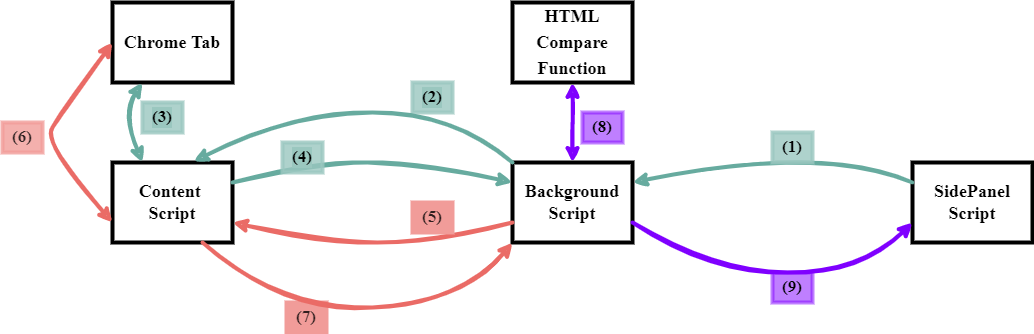
\includegraphics[width=1\textwidth]{picture/ch3-script-structure.png}
    \caption{擴充腳本之溝通流程圖}
    \label{f3.7}
\end{figure}

\subsection{SidePanel Script}\label{s3.4.1}
SidePanel Script是專門控制在Chrome Developer tools中Elements頁面旁子介面的腳本,
此腳本目前的主要功能在於若使用者點擊畫面中的互動按鈕或輸入相關字元,
會讓擴充元件執行相對應的行為。
如圖\ref{f3.7}中的(1)、(2)、(3)、(4)所示,
在UI介面下點擊開始比對的按鈕後,
等待第一個計時器結束後從Develope Tool中Elements Panel取出當下的HTML,
等待第二個計時器結束後再從Develope Tool中Elements Panel頁面取出當下的HTML,
共取出變更前以及變更後的兩個HTML。
取出後便開始與Background Script溝通讓它知道要開始進行比對了,
等到比對完後從Background Script得到結果並且把結果回傳給SidePanel Script,
最後將結果顯示在UI介面上,


\subsection{Background Script}\label{s3.4.2}
Background Script在擴充元件中的定位是在背景中執行的程式,開發者通常將此程式的主要邏輯撰寫在這腳本中,
而HTML比對腳本的函數也是在此腳本中執行的。
如圖\ref{f3.7}中的(5)、(6)、(7)所示,
接收到從SidePanel Script傳來的兩個HTML後便會開始比對,
並將最後的比對結果回傳到SidePanel Script中,



\section{UI/UX介面之實作}\label{s3.5}
設計此工具,為考慮人性化的使用介面以及比對後的結果方便使用者挑選所需要的條件,將此工具分成以下五個部分:
\subsection{Illustrate}\label{s3.5.1}
說明此擴充工具功能並且敘述該工具選擇的設定方式以及使用流程。

\subsection{Timer}\label{s3.5.2}
依照使用者當前的網路狀況、元件互動情況等等因素,藉由調整以下兩個Timer來調整抓取HTML的時間。

\begin{itemize}
    \item\textbf{Time Of Set Up: }
    在點擊``Start Compare''後,此Timer開始倒數計時,等時間結束後,便會抓取第一次的HTML。
    此Timer設計是為了讓使用者在點擊開始比對的按鈕後,
    有一段足夠的時間可以設置比對前的狀態,
    讓使用者保持在可控制的環境下執行比對功能。
    例如:使用者想要抓取元件從Hover狀態到沒有Hover狀態的變化過程,
    可以設定此Timer,讓使用者可以在點擊按鈕後有充足的時間將滑鼠Hover到該元件上。

    \item\textbf{Time Of Change Element: }
    等``Time Of Set Up''的時間結束並抓取第一次的HTML後,
    此Timer開始倒數計時,等時間結束後,
    便會將兩次的HTML一同傳送給Background Script執行比對。

\end{itemize}

\subsection{Options}\label{s3.5.3}

針對當前的使用情境,可以透過勾選以下選項,讓使用者過濾不需要的比對結果

    \begin{itemize}
        \item\textbf{Ignore style attribute's change: }
        在HTML中可以利用<style>標籤來建立簡易的CSS指令,但通常在使用時,較少用此標籤的內容當作路徑條件,
        為避免結果出現很多僅只有style屬性的變化,故可以勾選此條件來進行結果篩選。

        \item\textbf{Only display change of current selecting elemnt: }
        若當前的HTML結構過大,但使用者僅僅只是要查看當前節點的變化,顯示過多的變更結果會讓使用者較難找出適合的元件變化,
        為過濾掉當前節點之外的變更雜訊,在Develope Tool中Element頁面點擊HTML的節點,比較後的顯示結果僅會出現該節點的變化結果。
        
        \item\textbf{Display one tag's change: }
        為避免比較後顯示的結果過多,故添加了過濾元件tag的選項,
        讓使用者可以利用節點的tag過濾比對後的結果,例如:div、button等等類別。

    \end{itemize}

\subsection{Compare Control}\label{s3.5.4}

內部有兩個按鈕以及顯示比較情況的顯示框,可以點擊按鈕開始比對或點擊按鈕強制停止比對。

\subsection{Compare Result}\label{s3.5.5}

此面板中的下拉選單有顯示三種類型的結果:changed-area、added-area和removed-area,點擊後會出現表格顯示該節點的屬性比對,
內部表格顯示該節點所有屬性的before、after和diff比對結果。

\indent

\begin{figure}[H]
    \centering
    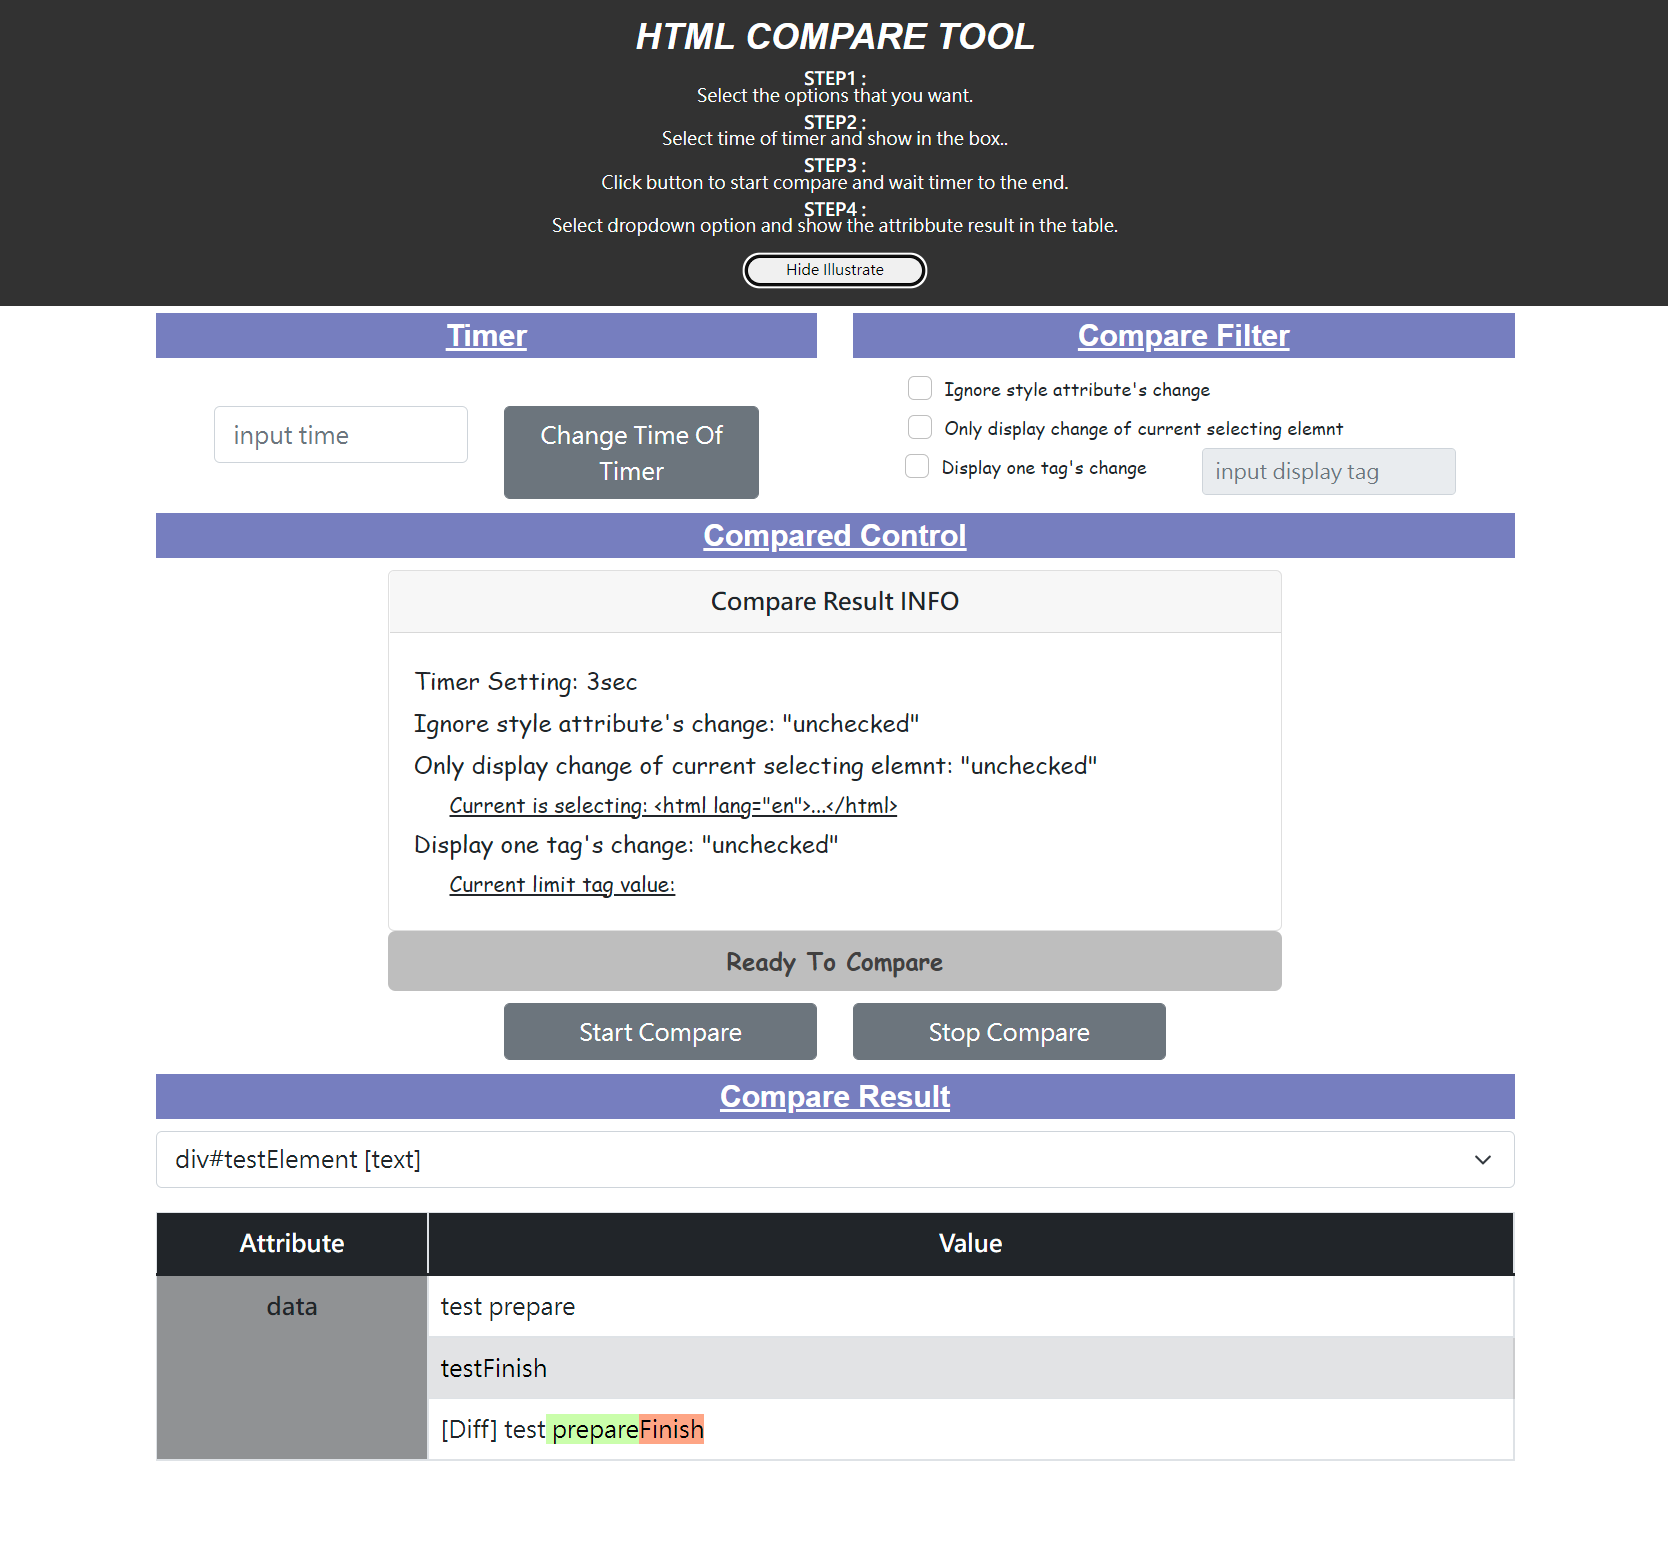
\includegraphics[width=0.9\textwidth]{picture/ch3-UIUX-example.png}
    \caption{UI設計之介面}
    \label{f3.8}
\end{figure}